\chapter{AFABL Programmer Study}\label{ch:programmer-study}

\section{Experiments}

Programmers will be randomly assigned to two equally-sized groups: one group will use Scala without AFABL first -- the Scala-first group -- and the other group will use Scala with AFABL first -- the AFABL-first group.  Each group will complete three programming tasks using Scala and AFABL in the order determined by their group.  For each task the programmers will be asked to design and implement elegant code that meets the requirements of the task as quickly as possible, balancing the quality of their solutions with time.  The idea is to get a good solution quickly, not a perfect solution in a long time.

\subsection{Task 1: The Bunny-Wolf Domain}\label{sec:task1}

\begin{figure}[h]

\begin{center}
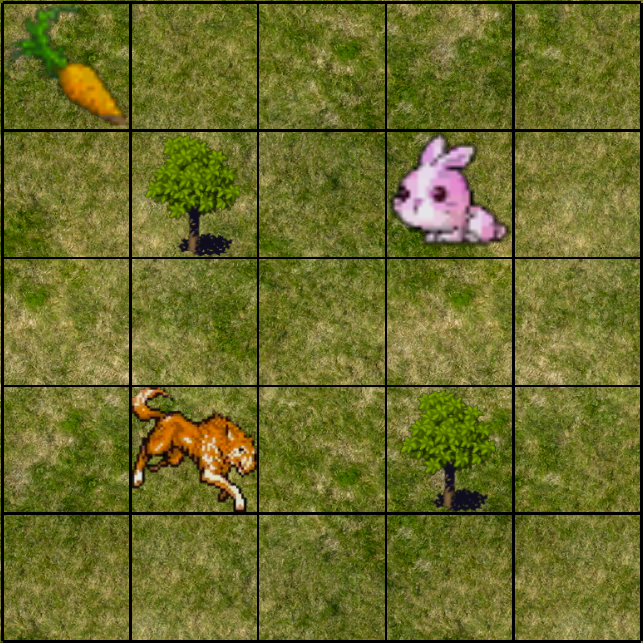
\includegraphics[height=2.4in]{bunny.png}
\end{center}


\caption{In the grid world above, the bunny must pursue two goals
  simultaneously: find food and avoid the wolf.  The bunny may move
  north, south, east, or west.  When it finds food it consumes the
  food and new food appears elsewhere in the grid world, when it meets
  the wolf it is eaten and ``dies.''}
\label{fig:bunny-picture}
\end{figure}

In this task each programmer will write an agent that controls a bunny character in a simple
world, depicted in Figure~\ref{fig:bunny-picture}.  The bunny world works as follows:

\begin{itemize}

\item The bunny world is a discrete grid of cells.  The bunny, wolf, and food each occupy one cell.

\item During each time step the bunny may move north, south, east, or west.

\item Every two time steps the wolf moves towards the bunny.

\item If the bunny moves to the cell currently occupied by the food, the bunny eats the food, receives a signal from the simulation that it has eaten the food, and new food appears elsewhere.

\item If the wolf moves to the cell currently occupied by the bunny it eats the bunny and the episode ends.

\end{itemize}

The simulation runs several episodes, keeping track of how much food the bunny eats and how long (how many time steps) the bunny ``lives'' in each episode.  Programmers will be asked to write bunny agents that live as long as possible and eat as much food as possible.

\subsection{Task 2: Mating Bunny}\label{sec:task2}

In this task each programmer will write a bunny agent for a world that is identical to the world in Task 1 except that the bunny must also find mates.  The world will include one static  potential mate that behaves similarly to the food.  When the bunny finds the potential mate, the bunny receives a signal that it has ``mated,'' the mate disappears (because it goes off to have babies), and another potential mate appears elsewhere.  The simulation runs as in Task 1, additionally keeping track of how many mates the bunny finds.  As in Task 1, programmers will be asked to write bunny agents that live as long as possible, eat as much food as possible, and find as many mates as possible.

\subsection{Task 3: Adding Wind, Spoiling Food, and Picky Mates}\label{sec:task3}

In this task each programmer will write a bunny agent for a world with the same elements as in Task 2 and with the same goals for the bunny, but the world is more complex.  In particular:

\begin{itemize}

\item There is constant wind from an unchanging direction that affects the wolf's ability to find the bunny.  The wolf will only move toward the bunny if the wolf is downwind of the bunny.

\item If food is not eaten within 15 time steps after it appears, it spoils.  Spoilage is represented by the food disappearing and new food appearing elsewhere.

\item To simulate selection of fit bunnies, potential mates will only accept the bunny if the bunny has eaten within 10 time steps (a hungry bunny is an unsuccessful bunny and therefore not fit for mating).  Rejection will be represented by the potential mate remaining in place and the bunny not receiving a signal that mating has occurred.

\end{itemize}



\section{Data Collection}

Data will be collected from programmers in three ways: directly through work diaries and surveys, and independently through static and dynamic analysis of programmers' submitted solutions to the programming tasks \cite{singer2008a-software}.  The following sections discuss each of the data collection methods.

\subsection{Programmer Demographics Survey}

The demographics survey will be given to participants after they have read and agreed to the consent form and before they are given task instructions and assigned to groups.

Purpose

The purpose of this survey is to place the programmers in groups according to their programming experience and skills.  In particular, the web application will use this survey to assign participants to the Scala-first and AFABL-first groups so that each group has similar distributions of programmer experience and skill levels.  Survey results may also be used to develop other quantitative and qualitative measures relating demographic information to task performance.

Questionnaire

\begin{enumerate}

\item What is your level of education?

\begin{enumerate}
\item High School
\item Associate Degree, or currently enrolled in Bachelor degree program
\item Bachelor Degree
\item Master Degree
\item Doctoral Degree
\end{enumerate}

Rationale: education level can affect programming proficiency.

\item What is your most applicable college major? By “most applicable” we mean the major you are using most in your profession. For example, if you got a B.S. in electrical engineering and a M.S. in computer science and work as a software engineer, then your most applicable major is computer science.

Rationale: college major can affect programming proficiency.  Additionally, we may code the data to distinguish between technical (but not necessarily computer science) and non-technical majors.

\item Number of years of professional programming experience. You may include years spent working on graduate research projects. Count a semester as .5 years.

Rationale: programming experience can affect programming proficiency.

\item Number of programming languages with which you have ever been proficient. Include only programming languages, not markup languages like XML/HTML, build specification languages like Make, or special purpose languages like Lex and Yacc.

Rationale: proficiency in multiple programming languages can affect can affect a programmer’s ability to use a new language/library.

\item Number of programming languages with which you are currently proficient.

Rationale: proficiency in multiple programming languages can affect can affect a programmer’s ability to use a new language/library.

\item How proficient are you with imperative programming (languages like C, C++, Java, Python) ?
\begin{enumerate}
\item Not proficient
\item Familiar (have done tutorials or simple examples)
\item Proficient (can write programs with multiple objects and files)
\item Expert
\end{enumerate}

Rationale: AFABL represents a novel programming paradigm.  Proficiency in multiple programming paradigms may affect a programmer’s ability to use AFABL.

\item How proficient are you at object-oriented programming (languages like Smalltalk, Ruby, Scala, Java, C++)? 

\begin{enumerate}
\item Not proficient
\item Familiar (have done tutorials or simple examples)
\item Proficient (can write programs with multiple objects and files)
\item Expert
\end{enumerate}

Rationale: AFABL represents a novel programming paradigm.  Proficiency in multiple programming paradigms may affect a programmer’s ability to use AFABL.

\item How proficient are you at functional programming (languages like Lisp/Scheme, Haskell, ML, Scala)? 

\begin{enumerate}
\item Not proficient
\item Familiar (have done tutorials or simple examples)
\item Proficient (can write programs with multiple objects and files)
\item Expert
\end{enumerate}

Rationale: AFABL represents a novel programming paradigm.  Proficiency in multiple programming paradigms may affect a programmer’s ability to use AFABL.

\item How proficient are you at game/agent programming? 

\begin{enumerate}
\item Not proficient
\item Familiar (have done tutorials or simple examples)
\item Proficient (can write programs with multiple objects and files)
\item Expert
\end{enumerate}

Rationale: game/agent programming proficiency is not common in the general programmer population.  Knowing programmers’ proficiency in game/agent programming will help randomize the experiment groups and allow additional inferences relating game/agent programming proficiency and proficiency with AFABL.

\item How proficient are you at Scala programming? 

\begin{enumerate}
\item Not proficient
\item Familiar (have done tutorials or simple examples)
\item Proficient (can write programs with multiple objects and files)
\item Expert
\end{enumerate}

Rationale: Scala is our baseline language, and AFABL is embedded in Scala.  Scala proficiency will have a profound effect on task proficiency and thus needs to be accounted for in randomizing the experiment groups.

\end{enumerate}

\subsection{Work Diary}

Programmers will be asked to record the total amount of time they spend in design and implementation for each task, the time they spend debugging, and the time they spend referring to documentation.

\subsection{Reflection Survey}

The purpose of the reflection survey is to develop a qualitative assessment of programmer satisfaction with AFABL.

Questionnaire

For each question, select the degree to which you agree with the statement based on
the agent programming tasks you completed for this experiment.

\begin{enumerate}
\item I have a positive impression of agent programming in AFABL.

\begin{enumerate}
\item Strongly disagree
\item Disagree
\item Neutral
\item Agree
\item Strongly Agree
\end{enumerate}

Rationale: programmers’ impression of Scala will provide a baseline for evaluating
programmers’ impression of AFABL.

\item I found it easier to write the agents using AFABL’s programming constructs compared to bare Scala.

\begin{enumerate}
\item Strongly disagree
\item Disagree
\item Neutral
\item Agree
\item Strongly Agree
\end{enumerate}

Rationale: the point of AFABL is to facilitate agent programming, so programmers should have a more positive impression of AFABL for agent programming.

\item I believe that AFABL facilitated more reusable and maintainable code for agents compared to bare Scala.

\begin{enumerate}
\item Strongly disagree
\item Disagree
\item Neutral
\item Agree
\item Strongly Agree
\end{enumerate}

Rationale: answers to this question should correlate with answers to Question 1.

\item If given the choice, I would choose AFABL over Scala for agent programming projects.

\begin{enumerate}
\item Strongly disagree
\item Disagree
\item Neutral
\item Agree
\item Strongly Agree
\end{enumerate}

Rationale: answers to this question should correlate with answers to Question 2.

\item I found it easier to use AFABL compared to Scala for Task 1.

\begin{enumerate}
\item Strongly disagree
\item Disagree
\item Neutral
\item Agree
\item Strongly Agree
\end{enumerate}

Rationale: in addition to objective analyses of task submissions, we want to know whether programmers subjectively prefer AFABL.

\item What was it about AFABL that made the Task 1 easier or harder?

Rationale: we want to get open-ended feedback for things we didn’t anticipate.

\item I found it easier to use AFABL compared to Scala for Task 2.

\begin{enumerate}
\item Strongly disagree
\item Disagree
\item Neutral
\item Agree
\item Strongly Agree
\end{enumerate}

Rationale: in addition to objective analyses of task submissions, we want to know whether programmers subjectively prefer AFABL.

\item What was it about AFABL that made the Task 2 easier or harder?

Rationale: we want to get open-ended feedback for things we didn’t anticipate.

\end{enumerate}

\section{Evaluation}

Using results from the pilot study, we will evaluate the internal consistency of the survey by calculating the Cronbach alpha coefficients for the following constructs:

\begin{enumerate}

\item User satisfaction with Scala for agent programming tasks.
\begin{itemize}
\item Questions 1 and 3
\end{itemize}

\item User satisfaction with AFABL for agent programming tasks.
\begin{itemize}
\item  Questions 2 and 4
\end{itemize}

\item User preference for AFABL over Scala for agent programming tasks.
\begin{itemize}
\item Questions 5 and 7
\end{itemize}

\end{enumerate}

The Cronbach alpha coefficient measures the correlation between the answers to questions that measure the same construct and is given by:

\[
\alpha = \frac{k}{k - 1} \times \frac{s_{T}^{2} - \sum s_{I}^{2}}{s_{T}^{2}}
\]

where
\begin{itemize}
\item $s_T^2$ is the total variance of all the items (questions) for a construct
\item $s_I^2$ is the variance of an individual item, and
\item $k$ is the number of items.
\end{itemize}

Typically a construct is considered valid if its Cronbach alpha coefficient is at least 0.7.



\section{Source Code Analysis}

The code submitted for each task will be analyzed to determine:

\begin{itemize}
\item How much code was required for each task with and without AFABL.
\item How consistent the solutions were between programmers in each task with and without AFABL.  Did AFABL lead to more consistent designs?
\item How well the programmers understood the problem.
\end{itemize}

\section{Run-time Analysis}

The performance of the solutions submitted for each task will be recorded using repeated trials.  In essence, each solution will compete with the others.

\subsection{Logistics}

The experiments will be conducted online to provide easy access to the greatest number of participants.  Participants will:

\begin{enumerate}
\item Register online with confidential identifying information.
\item Complete demographics survey.  The web application will use the demographic survey to place participants in the Scala-first or AFABL-first groups.
\item Download code and task instructions.
\item Complete Task 1 in Scala and AFABL.
\item Submit Task 1 solutions, including work diary.
\item Complete Task 2 in Scala and AFABL.
\item Submit Task 2 solutions, including work diary.
\item Complete Task 3 in Scala and AFABL.
\item Submit Task 3 solutions, including work diary.
\item Complete experiment reflection survey.
\end{enumerate}

The entire experiment will be designed to take less than 20 hours to complete.

\subsection{Contingency Plans}

In the event that an insufficient number of online participants can be recruited, we will hold in-person workshops with students from Georgia Tech, lured by free pizza and free Scala training (since Scala use is relatively low at Georgia Tech).

\section{Evaluation}

The primary quantitative metric will be task completion effort in time and code quantity.  Tasks 2 and 3 will provide a measure of how much effort is required to adapt agents to new domains.  In addition, we will calculate qualitative metrics for programmer satisfaction, and mine the source code for design patterns.
